\documentclass[a4paper]{article}

\usepackage{physics}
\usepackage{pdfpages}
\usepackage{bm}
\usepackage{tikz}
\usetikzlibrary{matrix,shapes,arrows,positioning,chains,calc}
\usepackage{lscape}
\usepackage[english]{babel}
\usepackage[utf8]{inputenc}
\usepackage{amsmath}
\usepackage[top=1in, bottom=1.25in, left=1in, right=1in]{geometry}
\usepackage{fancyhdr}
\setlength{\headheight}{15.2pt}
\pagestyle{fancy}
\usepackage{hyperref}
\usepackage{float}
\usepackage{graphicx}
\usepackage{caption}
\usepackage{subcaption}
\usepackage{wrapfig}
\usepackage{color}
\usepackage{dsfont}
\usepackage{color, colortbl}

\newcommand{\HRule}{\rule{\linewidth}{0.5mm}}

\lhead{Simon Hudson}
\chead{PHYC30012}
\rhead{22-10-2016}

\begin{document}

\begin{center}
\textsc{\Large PHYC30012 Computational Physics}\\[0.3cm]

\HRule \\[0.4cm]

{\LARGE \bfseries Project 5 - A Fiery Death and State-Based Estimation \\[0.4cm] }
{\Large 22nd October 2016 \\}

\HRule \\[0.3cm]

{\large Simon Hudson 767507\\[0.5cm]}

\end{center}

\section{Introduction}
This project deals with the so-called Kalman filter, an algorithm for a recursive solution to the discrete-data linear filtering problem. Originally published in a 1960 paper by R.E. Kalman, the algorithm provides an efficient recursive computational means to estimate the state of a process, in a way that minimises the mean of the squared error (or variance)\cite{Manual}.

\section{Background}\label{Background}
	\subsection{Parameter estimation}\label{Parameter_estimation}
		We will be considering the measurement of a random variable y given by:
		\begin{align}
			y(t)=x(t,\bm{\vec{\theta}}) + \nu(t)\label{Underlying_process_equ}
		\end{align}
		\noindent where y is the measured value of an underlying process, x is the true value, and $\nu$ is a stochastic random variable modelling the error in the measurements. The vector $\bm{\vec{\theta}}$ contains the parameters of the process x. Using the best unbiased estimator, we would find that our estimate of $\bm{\vec{\theta}}$ approaches the true value of $\bm{\vec{\theta}}$ as the number of measurements becomes large.

	\subsection{Covariance}\label{Covariance}
		For vectors of zero-mean random variables:
		\begin{align}
			\begin{bmatrix}
				X_{1}\\
				X_{2}\\
				\hdotsfor{1} \\
				X_{n}
			\end{bmatrix}
		\end{align}
		
		\noindent We form the covariance matrix as follows:
		
		\begin{align} \label{Covariance_matrix}
			\begin{bmatrix}
				E[X_1X_1] & E[X_1X_2] & E[X_1X_3] & \dots  & E[X_1X_4] \\
				E[X_2X_1] & E[X_2X_2] & E[X_2X_3] & \dots  & E[X_2X_4] \\
				\vdots & \vdots & \vdots & \ddots & \vdots \\
				E[X_nX_1] & E[X_nX_2] & E[X_nX_3] & \dots  & E[X_nX_n] \\
			\end{bmatrix}
		\end{align}
		
		\noindent Where:
		
		\begin{align} \label{Covariance_equ}
			E[X_iX_j]=\frac{1}{N-1}\sum_{k}(x_{ik}-\overline{x}_i)(x_{jk}-\overline{x}_j)
		\end{align}
		
		\noindent and $x_{ik} \in X_i, x_{jk}\in X_j$ are sets of N random variables, $\overline{x}_i$ is the mean of $X_i$, and $\overline{x}_j$ is the mean of $X_j$.\\
		
		\noindent The elements of the leading diagonal of this matrix are just the variances of the corresponding random variables $X_1, X_2, \dots X_n$.
	
	\subsection{The Kalman filter}\label{The_Kalman_filter}
	The calculation of the general case of k measurements with n dimensions involves computing the inverse of a $kn \times kn$ matrix, the computational time for which grows $\propto k^3$. To get around this we can incorporate the measurements sequentially, using the discrete time Kalman filter update equations. Here measurements are taken at time intervals $\Delta t$, indexed by k such that $t=\Delta t \times k$. At each step we use the Kalman filter equations (section \ref{System_dynamics}) to update our state estimate $\bm{\vec{\theta}}$.
		\subsubsection{Definitions}\label{Definitions}
		$\bm{\vec{\theta}}_{k|k-1}$ represents our best estimate of $\bm{\vec{\theta}}$ at measurement k given k-1 samples, and $\bm{P}_{k|k-1}$ is the covariance matrix for the estimate $\bm{\vec{\theta}}_{k|k-1}$. $\bm{m}_k$ is a vector of all measured quantities for the $k^{th}$ measurement and $\bm{v}_k$ is a vector of random variables representing the error on those quantities, given by covariance matrix $\bm{R}$. Thus the underlying process we are modelling, as per equation \ref{Underlying_process_equ} is given by:
		\begin{align}
			\bm{m}=\bm{H\theta}+\bm{v}
		\end{align}
	
		\noindent  We have introduced the 'propagation matrix' $\bm{H}$ given by:
		
		\begin{align}
		\bm{H}=
		\begin{bmatrix}
		1 & 0 & cos(wt) & 0 \\
		0 & 1 & 0 & sin(wt) \\
		\end{bmatrix}
		\end{align}
		
		\noindent and state estimate:
		
		\begin{align}
		\bm{\vec{\theta}}=\begin{bmatrix}
			x_0\\
			y_0\\
			A \\
			B
		\end{bmatrix}
		\end{align}
		
		\subsubsection{Final result}\label{Final_result}
		Thus the final result of our estimation will be given by:
		\begin{align}
			\bm{\vec{z}}=\bm{H\theta}
		\end{align}
		\noindent or
		\begin{align}
			z_x=x_0+Acos(wt)\\
			z_y=y_0+Asin(wt)
		\end{align}
		\noindent which are the required equations of an ellipse, centred on the point $(x_0, y_0)$ parametrised in time with angular frequency $w$.
	
\clearpage
\section{Method and results}\label{Method_results}
	\subsection{Parameter choices}\label{Parameter_choices}
		All distances are given in units of $10^7 km$ and time expressed in $years$.
		\subsubsection{Variables given}\label{Variables_given}
		We are given that angular frequency of the asteroid orbit, $w=0.2625$, and that the planet is located at coordinates $\vec{p}=(-0.1, 1.3)$ with radius $r_p=0.02$.\\

		\noindent Here we have chosen the following initial values:
		\begin{align}
			\bm{\vec{\theta}}_{0|-1}=
			\begin{bmatrix}
				2\\
				2\\
				2\\
				2\\
			\end{bmatrix}
		\end{align}
		\begin{align}
			\bm{P}_{0|-1}=
			\begin{bmatrix}
			0.1	&	0 	&	0 & 	0 \\
			0 &		0.1 &	0 &		0 \\
			0 &		0 &		0.1 &	0 \\
			0 &		0 &		0 &		0.1 \\
			\end{bmatrix}
		\end{align}
		Here we have chosen a diagonal matrix for $\bm{P}$, representing state vectors $\bm{\vec{\theta}}$ whose individual variances are 0.1 and whose elements are uncorrelated.
		
		\subsubsection{Measurement covariance matrix}\label{Measurement_covariance_matrix}
			\noindent Since the noise processes are known to be Gaussian, independent among samples and state variables, with zero mean and variance of $0.06^2=0.0036$, the covariance matrix for the measurements was set:
			\begin{align}
				\bm{R}=
				\begin{bmatrix}
				0.0036 & 0 \\
				0 & 0.0036 \\
				\end{bmatrix}
			\end{align}
			
		\subsubsection{Time measurement}\label{Time_measurement}
			\noindent In the discrete time Kalman filter update equations, the time interval is given by:
			\begin{align}
				\Delta t=\frac{1}{2000}
			\end{align}

			\noindent Since we are given that $t_i=2\pi$, the time at any point is given by:
			\begin{align}
				t=2\pi+\frac{1}{2000} \times k \label{Time_equ}
			\end{align}
				
			\noindent and we are given an upper bound of $t_f=3\pi$.
			
		\subsubsection{Measurements}\label{Measurements}
			Data is read in from separate data files for x and y values, and for each successive cycle k of the loop, assigned to the measurement vector as follows:
			\begin{align}
				\bm{m}_k=
				\begin{bmatrix}
					x_k \\
					y_k \\
				\end{bmatrix}
			\end{align}

	\subsection{System dynamics}\label{System_dynamics}
	
		\noindent The equations governing the dynamics of the system are as follows:
			\begin{align}
				\bm{\vec{\epsilon}_k}=\bm{\vec{m}_k}-\bm{H_k\vec{\theta}_{k-1}}\label{Kalman_residuals}
			\end{align}
			\begin{align}
				\bm{S_k}=\bm{H_kP_{k-1}H_k^T} + \bm{R}
			\end{align}
			\begin{align}
				\bm{K_k}=\bm{P_{k-1}H_k^TS_k^{-1}}
			\end{align}
			\begin{align}
				\bm{\vec{\theta}_k}=\bm{\vec{\theta}_{k-1}}+\bm{K_k\vec{\epsilon}_k}
			\end{align}
			\begin{align}
				\bm{P_k}=(\bm{\mathds{1}}-\bm{K_kH_k})\bm{P_{k-1}}\label{Kalman_est_covariance}
			\end{align}
			\begin{align}
				k = k+1
			\end{align}
		
		\noindent The matrix $\bm{S}_k$ is the covariance in the residuals $\bm{\vec{\epsilon}}_k$. That is, $\bm{S}_k$ is the covariance of the distributions for which the elements of $\bm{\vec{\epsilon}}_k$ are the means. \\
		
		\noindent The Kalman gain $\bm{K_k}$ is the constant of proportionality by which we multiply the residuals $\bm{\vec{\epsilon}}$ to then add to our previous state estimate $\bm{\vec{\theta_{k-1}}}$ to update it to the new state estimate $\bm{\vec{\theta_{k}}}$. It is a measure of how worried we should be about the differences between our model and the measurement.\\
		
		\noindent The matrix $\bm{P}_{k|k-1}$ represents the covariance of the distribution for which the elements of the current estimate $\bm{\vec{\theta}}_{k|k-1}$ are the means. $\bm{\vec{\theta}}$ and $\bm{P}$ are updated at the end of each cycle thus:
		\begin{align}
			\bm{P}_{k|k-1}=\bm{P}_{k|k}\\
			\bm{\vec{\theta}}_{k|k-1}=\bm{\vec{\theta}}_{k|k}
		\end{align}
	
	
	\subsection{Changes in state parameters}
	As the number of measurements increases:
		\begin{enumerate}
			\item The state estimate $\bm{\vec{\theta}}$ moves closer and closer to the true value representing the underlying process that we are modelling.
			\item The elements of the residuals matrix $\bm{\vec{\epsilon}}$ decrease in magnitude, representing a decrease in the difference between what we expect to see and what we measure.
			\item The elements of the residuals covariance matrix $\bm{S}$ decrease in magnitude, representing a decrease in the covariance of the residuals. That is, as time goes on, the residuals are more centred on their mean, with less spread, and less correlation between the distributions that each element of $\bm{\vec{\epsilon}}$ represents.
			\item The elements of the Kalman gain $\bm{K}$ decrease in magnitude, very rapidly at first, then tapering off as $\bm{\vec{\theta}}$ approaches the best estimate.
			\item The diagonal elements of the estimate covariance $\bm{P}$ decrease in magnitude, indicating that the variance of each distribution of which the elements of $\bm{\vec{\theta}}$ are the mean decreases. The off-diagonal elements of $\bm{P}$ increase from zero to small final magnitudes, indicating an increase in correlation between the distributions represented by the different elements of $\bm{\vec{\theta}}$. See section \ref{Final_value_of_P} for further discussion of this.
		\end{enumerate}
	
	\subsection{First iteration of Kalman filter}\label{First iteration of Kalman filter}
		For the first iteration, equation \ref{Kalman_residuals} becomes:
		\begin{align}
			\bm{\vec{\epsilon}_0}=\bm{\vec{m}_0}-\bm{H_0\vec{\theta}_{0|-1}}\\
		\end{align}
		Analytically (to 4 significant figures since $w$ is only provided to that accuracy):
		\begin{align}
			\bm{\vec{\epsilon}_0}=
			\begin{bmatrix}
				1.130263204 \\
				2.733042777 \\
			\end{bmatrix}-
			\begin{bmatrix}
				1 &	0 &	cos(wt_i) &	0 \\
				0 &	1 &	0 &	sin(wt_i) \\
			\end{bmatrix}
			\begin{bmatrix}
				2 \\
				2 \\
				2 \\
				2 \\
			\end{bmatrix}
		\end{align}
		\begin{align}
			\Rightarrow\bm{\vec{\epsilon}_0}=
			\begin{bmatrix}
				1.130263204 \\
				2.733042777 \\
			\end{bmatrix}-
			\begin{bmatrix}
				1 &	0 &	-0.07846 &	0 \\
				0 &	1 &	0 &				0.9969 \\
			\end{bmatrix}
			\begin{bmatrix}
				2 \\
				2 \\
				2 \\
				2 \\
			\end{bmatrix}
		\end{align}
		\begin{align}
			\Rightarrow\bm{\vec{\epsilon}_0}=
			\begin{bmatrix}
				1.130263204 \\
				2.733042777 \\
			\end{bmatrix}-
			\begin{bmatrix}
				1.843 \\
				3.994 \\
			\end{bmatrix}
		\end{align}
		\begin{align}
			\Rightarrow\bm{\vec{\epsilon}_0}=
			\begin{bmatrix}
				-0.7127 \\
				-1.261 \\
			\end{bmatrix}(4 sig. figs.)
		\end{align}
		Computationally the result was:
		\begin{align}
			\bm{\vec{\epsilon}_0}=
			\begin{bmatrix}
				-0.71281866 \\
				-1.26079189 \\
			\end{bmatrix}
		\end{align}
		We can see the results are quite accurate to the four significant figures provided in the $w$ value, only being out in the x coordinate by $1\times 10^{-4}$ units (where the units are $10^7km$).

	\clearpage
	\tikzstyle{startstop} = [rectangle, rounded corners, minimum width=3cm, minimum height=1cm,text centered, draw=black, fill=red!30]
	\tikzstyle{io} = [trapezium, trapezium left angle=70, trapezium right angle=110, minimum width=3cm, minimum height=1cm, text centered, draw=black, fill=blue!30]
	\tikzstyle{process} = [rectangle, minimum width=3cm, minimum height=1cm, text centered, draw=black, fill=orange!30]
	\tikzstyle{decision} = [diamond, minimum width=3cm, minimum height=1cm, text centered, draw=black, fill=green!30]
	\tikzstyle{arrow} = [thick,->,>=stealth]
	
	\begin{figure}
		\subsection{Flowchart}\label{Flowchart}
		\centering
		\caption{Flowchart for the computational implementation of a discrete time Kalman filter.} \label{Fig_flowchart}
		\begin{tikzpicture} [
			start chain,
			node distance=3mm,
			inner sep=5pt,
			text width=10cm,
			auto
		]
			\node (start) [
				startstop,
				draw,
				on chain=going below,
				join
			] {
				Start
			};
			\node (accept) [
				io,
				below of=start,
				draw,
				on chain=going below,
				join
			] {
				Accept input parameters as per section \ref{Parameter_choices}:\\
				Ellipse period $w$, location of planet $\vec{p}$, radius of planet $r_p$, initial state vector estimate $\bm{\vec{\theta}}_{0|-1}$, initial estimate covariance $\bm{P}_{0|-1}$, measurement covariance $\bm{R}$, inital time $t_i$, final time $t_f$, time increment $\Delta t$
			};
			\node (read-input) [
				io,
				below of=accept,
				draw,
				on chain=going below,
				join,
				text width=9cm
			] {
				Read in measurements from file into array, to be used stepwise for the elements of $\bm{\vec{m}}$.\\
			};
			\node (iterate) [
				process,
				below of=read-input,
				draw,
				on chain=going below,
				join
			] {
				Run all matrix operations in Kalman filter (equations \ref{Kalman_residuals} - \ref{Kalman_est_covariance})
			};
			\node (update) [
				process,
				below of=read-input,
				draw,
				on chain=going below,
				join
				] {
					Update the state vector and its covariance as follows:\\
					$\bm{\vec{\theta}}_{k|k-1}=\bm{\vec{\theta}_{k|k}}$\\
					$\bm{\vec{P}}_{k|k-1}=\bm{\vec{P}_{k|k}}$\\
					Update time as per equation \ref{Time_equ}
			};
			\node (store-and-check) [
			process,
			below of=update,
			draw,
			on chain=going below,
			join
			] {
				Calculate the trace of $\bm{\vec{P}}_{k|k-1}$, and the current value of $t_k$ and store in arrays for plotting\\
				Store the current values of measurements $\bm{\vec{m}}_k$ for plotting\\
			};
			\node (test) [
				decision,
				below of=store-and-check,
				draw,
				on chain=going below,
				join,
				text width=3cm,
			] {
				Is current time $t_k<3\pi$?
			};
			\node (plot) [
				process,
				below of=thermalise,
				draw,
				on chain=going below,
				join
			] {
				Plot a scatter plot of the asteroid measurements, along with an ellipse representing the final values for $\bm{\vec{\theta}}$. Also plot ellipses for alternative trajectories of the asteroid, taking the values of $\bm{\vec{\theta}}$ plus or minus one standard deviation in the appropriate direction to give the largest possible deviation from the path represented by the mean values. If the asteroid poses a threat, mark the time and coordinates of anticipated collision.\\
				Plot a line representing the trace of $\bm{\vec{P}}$ versus time $t_k$
			};
			\node (stop) [
				startstop,
				below of=plot-mag-beta,
				draw,
				on chain=going below,
				join
			] {
				Stop
			};
				
			\draw [arrow] (start) -- (accept);
			\draw [arrow] (accept) -- (read-input);
			\draw [arrow] (read-input) -- (iterate);
			\draw [arrow] (iterate) -- (update);
			\draw [arrow] (update) -- (store-and-check);
			\draw [arrow] (store-and-check) -- (test);
			\draw [arrow] (test) -- ($(test.east)+(1.5,0.0)$) node[below,pos=0.7, text width=2cm] {Yes} -| ($(iterate.east)+(1.5,0.0)$) -- (iterate.east);
			\draw [arrow] (test) -- (plot) node[right,pos=0.3, text width=2cm] {No};
			\draw [arrow] (plot) -- (stop);
			
		\end{tikzpicture}
	\end{figure}

	\clearpage
	\subsection{Estimate of state vector and covariance}\label{Estimate_of_state_vector_and_covariance}
	The final state vector was computed using the implementation in figure \ref{Fig_flowchart} as follows:
	\begin{align}
		\bm{\vec{\theta}}_{final}=\begin{bmatrix}
			(x_0)_{final}\\
			(y_0)_{final}\\
			A_{final} \\
			B_{final} \\
		\end{bmatrix}=
		\begin{bmatrix}
			1.20130262 \\ 
			1.10099351 \\
			1.30164666 \\
			1.69819068 \\
		\end{bmatrix}
	\end{align}
	The final covariance matrix $\bm{P}$ was computed as follows:
	\begin{align}\label{Final_P_matrix}
		\bm{P}_{final}=
		\begin{bmatrix}
			0.00000338 & 	0.00000000 &	0.00000614 &	0.00000000 \\
			0.00000000 &	0.00003379 &	0.00000000 &	-0.00003875 \\
			0.00000614 &	0.00000000 &	0.00001340 &	0.00000000 \\
			0.00000000 &	-0.00003875 &	0.00000000 &	0.00004521 \\
		\end{bmatrix}
	\end{align}
	Therefore the variance in $x_0$ is 0.00000338, in $y_0$ is 0.00003379, in $A$ is 0.00001340, and in $B$ is 0.00004521.\\

	\subsection{How variance changes for different initial conditions}\label{How_variance_changes_for_different_initial_conditions}
	The values used within the initial conditions for $\bm{\vec{\theta}}_{0|-1}$, $\bm{P}_{0|-1}$ and $\bm{R}$ were varied independently over at least four orders of magnitude. The baseline values are highlighted in grey in the table.
	\begin{table}[h!]
		\centering
		\begin{tabular}{| c c c c | c | c | c c c c |}
			\hline
			\multicolumn{4}{|c|}{$\bm{\vec{\theta}}_{0|-1}$} & $\bm{P}_{0|-1}$ & $\bm{R}$ & \multicolumn{4}{|c|}{$\bm{P}_{final}$} \\
			$x$ & $y$ & $A$ & $B$ & diag. val. & diag. var. & $\sigma_{11}$ & $\sigma_{22}$ & $\sigma_{33}$ & $\sigma_{44}$ \\
			\hline
			0.02 &	0.02 &	0.02 &	0.02 &	0.1 &	0.0036 &	0.00000338 &	0.00003379 &	0.00001340 &	0.00004521 \\
			0.2 & 	0.2 &	0.2 & 		0.2 &		0.1 &	0.0036 &	0.00000338 &	0.00003379 &	0.00001340 &	0.00004521 \\
			\rowcolor{gray!30} 2 &		2 &			2 &			2 &			0.1 &	0.0036 &	0.00000338 &	0.00003379 &	0.00001340 &	0.00004521 \\
			20 &	20 &	20 &		20 &		0.1 &	0.0036 &	0.00000338 &	0.00003379 &	0.00001340 &	0.00004521 \\
			200 &	200 &	200 &	200 &	0.1 &	0.0036 &	0.00000338 &	0.00003379 &	0.00001340 &	0.00004521 \\
			2000 &	2000 &	2000 &	2000 &	0.1 &	0.0036 &	0.00000338 &	0.00003379 &	0.00001340 &	0.00004521 \\
			20000 &	20000 &	20000 &	20000 &	0.1 &	0.0036 &	0.00000338 &	0.00003379 &	0.00001340 &	0.00004521 \\
			\hline
			2 &		2 &			2 &			2 &			0.001 &	0.0036 &	0.00000334 &	0.00003136 &	0.00001319 &	0.00004195 \\
			2 &		2 &			2 &			2 &			0.01 &	0.0036 &	0.00000338 &	0.00003355 &	0.00001338 &	0.00004489 \\
			2 &		2 &			2 &			2 &			1.0 &	0.0036 &	0.00000339 &	0.00003381 &	0.00001340 &	0.00004524 \\
			2 &		2 &			2 &			2 &			10.0 &	0.0036 &	0.00000339 &	0.00003381 &	0.00001340 &	0.00004524 \\
			\hline
			2 &		2 &			2 &			2 &			0.1 &	0.00000036 &	0.00000000 &	0.00000000 &	0.00000000 &	0.00000000 \\
			2 &		2 &			2 &			2 &			0.1 &	0.000036 &		0.00000003 &	0.00000034 &	0.00000013 &	0.00000045 \\
			2 &		2 &			2 &			2 &			0.1 &	0.36 &				0.00033369 &	0.00313580 &	0.00131854 &	0.00419506 \\
			2 &		2 &			2 &			2 &			0.1 &	36.0 &				0.01507278 &	0.03972218 &	0.05141824 &	0.05219436 \\
			\hline  
		\end{tabular}
		\caption{Table of how variance of $\bm{\vec{\theta}}$ changes for different initial conditions.}\label{Tab_var_changes}
	\end{table}

	\noindent It is clear that the variance in the parameters has very little dependence on the initial value of $\bm{\vec{\theta}}_{0|-1}$. There was no change even though the initial value was changed over six orders of magnitude. The variance in the parameters also has very little dependence on $\bm{P}_{0|-1}$, after changing over four orders of magnitude. The biggest change observed was a 7.2107941\% change in $\sigma_{44}$ as compared to the baseline values.\\
	
	By contrast, it is clear that the variance in the parameters has a strong dependence on the values used on the principle diagonal of $\bm{R}$. We observe changes as large as 445840.24\% in $\sigma_{11}$ as compared to the baseline values. We would expect this, since the larger the values of the elements of $\bm{R}$, the higher the covariances of the noise present in the measurements, and hence the harder it will be to make an accurate prediction of the parameters of the underlying process. Under these circumstances we would expect higher final variances of the distributions for which the elements of $\bm{\vec{\theta}}$ represent the means.

	\clearpage
	\subsection{Plots}\label{Plots}
	\begin{figure}[ht!]
		\centering
		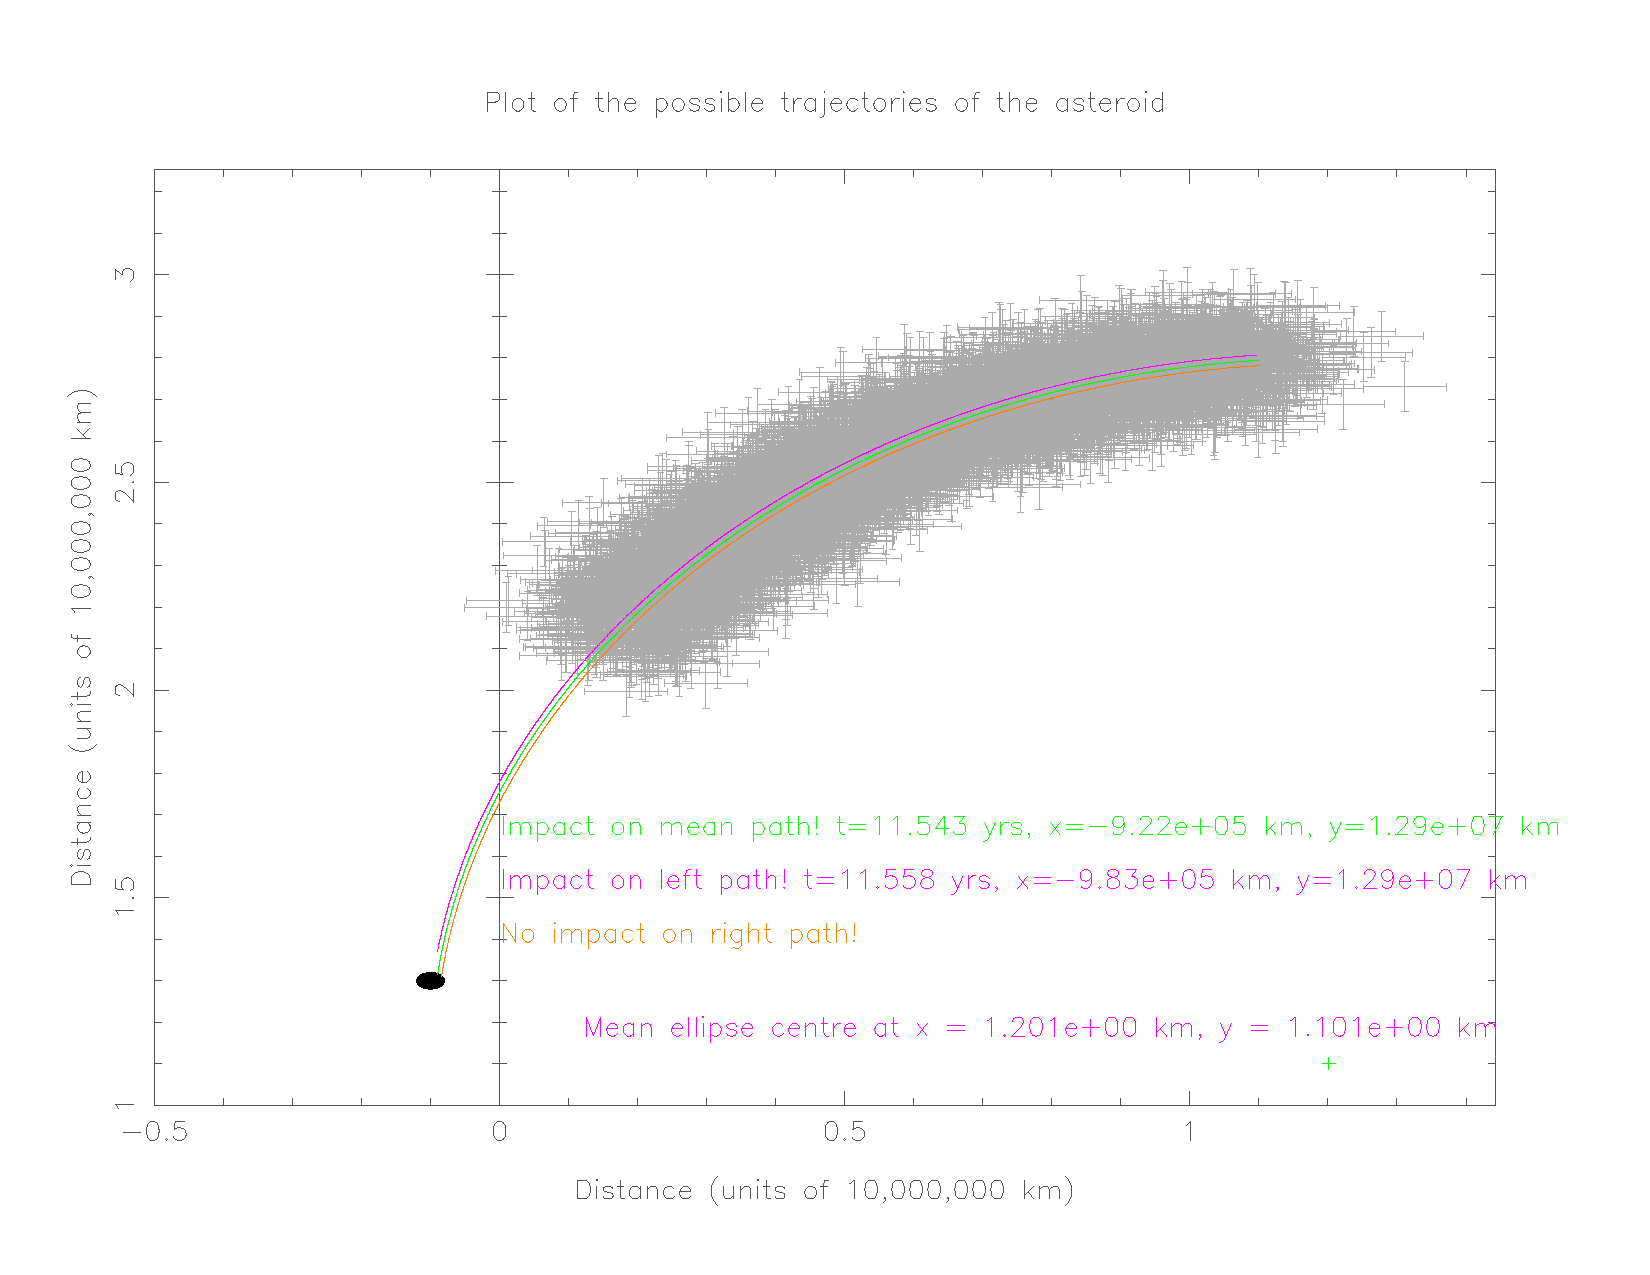
\includepdf[pages=1]{plots/proj5plot.pdf}
		\caption{Plot of the trajectory of the asteroid showing measurement data points with error bars, the final ellipse calculated, and whether impact is predicted.}\label{Fig_traj}
	\end{figure}
	\noindent For the mean path (marked in green), it is clear that impact is predicted. For more analysis see section \ref{Salvation}.
	
	\clearpage
	\subsection{The trace of P}\label{Trace_of_P}
	The final value of the trace of the estimate covariance matrix $\bm{P}$, tr($\bm{P}$) is 0.00009577.\\
	
	tr($\bm{P}$) represents the sum of the variances of all the elements of the estimate $\bm{\vec{\theta}}$. Therefore it is a indication the overall variance present in $\bm{\vec{\theta}}$. It can also be seen as the sum of the eigenvalues of the $\bm{P}$ matrix\cite{Wiki_trace}, or as the average squared distance to the centroid of the distribution that it represents\cite{Stack_exch__trace}.\\
	
	This implies that it may be possible that the asteroid may not hit the planet after all, because there is small but non-zero variance in the values of $\bm{\vec{\theta}}$. Therefore there is room for error, and the final values of the underlying process may not be exactly the means of their values as indicated by $\bm{\vec{\theta}}$ alone. In fact we find this is the case. \\
	
	\subsection{Room for salvation?}\label{Salvation}
	Plotted on figure \ref{Fig_traj} are also paths representing ellipses drawn using values changed by one standard deviation (the square root of the variances on the leading diagonal of $\bm{P}$) from the mean values taken from $\bm{\vec{\theta}}$. These standard deviations were added or subtracted from the mean values of $x_0$, $y_0$, $A$ and $B$ so as to construct ellipses representing the furthest paths the asteroid could reasonably take that might miss the planet on either the left or the right hand side, thus:
	\begin{align}
		x_{left}=(x_{0})_{smallest}+A_{largest}cos(wt)\\
		y_{left}=(y_{0})_{largest}+A_{largest}sin(wt)
	\end{align}
	\begin{align}
		x_{right}=(x_{0})_{largest}+A_{smallest}cos(wt)\\
		y_{right}=(y_{0})_{smallest}+A_{smallest}sin(wt)
	\end{align}
	
	 As the labels in the figure show, the mean and 'left' ellipses both impact the planet, whereas the 'right' ellipse does not. An error in plotting seems to show that the 'right' ellipse will also impact, but the values themselves used during calculation indicate this is not the case. Therefore there is a reasonable possibility that the asteroid may miss the planet.

	\subsection{The final value of P}\label{Final_value_of_P}
	The final value of $\bm{P}$ is repeated here for convenience:
	\begin{align}\label{Final_P_matrix_2}
		\bm{P}_{final}=
		\begin{bmatrix}
		0.00000338 & 	0.00000000 &	0.00000614 &	0.00000000 \\
		0.00000000 &	0.00003379 &	0.00000000 &	-0.00003875 \\
		0.00000614 &	0.00000000 &	0.00001340 &	0.00000000 \\
		0.00000000 &	-0.00003875 &	0.00000000 &	0.00004521 \\
		\end{bmatrix}
	\end{align}
	
	\noindent The extra information this contains over $tr(\bm{P})$ is the covariance of each element of the state vector $\bm{\vec{\theta}}$ with each other element. This is contained in the off-leading-diagonal elements, in the way shown in equations \ref{Covariance_matrix} and \ref{Covariance_equ}.\\
	
	Therefore we see:
	\begin{align}
		E[X_1X_3]=E[x_0A]=0.00000614\\
		E[X_2X_4]=E[y_0B]-0.00003875
	\end{align}
		(and, since covariance matrices are always symmetric)
	\begin{align}
		E[X_3X_1]=E[Ax_0]=0.00000614\\
		E[X_4X_2]=E[By_0]=-0.00003875
	\end{align}
	
	We expect $\bm{P}$ to be of this form because we would expect the values of $\bm{\vec{\theta}}$ to end up with some slight small dependence on each other. Here we can see that there is a correlation between the values relating to the x-coordinate, $x_0$ and $A$, and those relating to the y-coordinate, $y_0$ and $B$ (as well as the converse, between $A$ and $x_0$, and $B$ and $y_0$). This is expected because they have a close relationship, being related to the same coordinate axis, and the filter will have a harder time disassociating them from each other.
	
	\clearpage
	\subsection{Plot of the trace of P}\label{Plot_trace_of_P}
	\begin{figure}[ht!]
		\centering
		\includepdf[pages=2]{plots/proj5plot.pdf}
		\caption{Plot of tr($\bm{P}$) versus time.}\label{Fig_tr_P_plot}
	\end{figure}	
	
	\clearpage
	\subsection{The trace of P}\label{Trace_of_P_plot}
	As the number of measurements increases, $tr(\bm{P})$ decreases, as shown in figure \ref{Fig_tr_P_plot}. We would expect this, since $tr(\bm{P})$ is the sum of the variances of the elements of $\bm{\vec{\theta}}$. Therefore as time goes on and more measurements are made, our estimate for $\bm{\vec{\theta}}$ improves in accuracy compared to the true value of the underlying process, hence the variance of its elements will decrease.

\clearpage
\section{Conclusion}
We have created a program to implement the discrete time Kalman filter, in modelling the trajectory of an asteroid to predict whether it will impact an inhabited planet.\\

Our predictions indicate it is most likely that the asteroid will impact the planet, derived using the final estimate for the state vector $\bm{\vec{\theta}}$, containing the mean values of the distribution that it represents. However there is a statistically significant possibility, calculated using values of the distribution within one standard deviation of the mean, that the asteroid will not impact. With further analysis, it may be possible to derive a probability for impact.\\

The variance in the final estimate was shown to be very robust with choice of initial values of $\bm{\vec{\theta}}$ and $\bm{P}$, but sensitive to the variance of the noise present in the measurements, given by the leading diagonal elements of $\bm{R}$.\\

The trace of $\bm{P}$ was plotted, showing that it decreases as time goes on and more measurements are made.\\

We found that the final values of $\bm{\vec{\theta}}$ are correlated to a small extent, but only between values that relate to the same coordinate axis, for example between $x_0$ and $A$, and between $y_0$ and $B$ (and vice versa).

\begin{flushleft}
	\begin{thebibliography}{99}
			\bibitem{Manual}
			PHYC30012 Computational Physics manual
			\bibitem{Wiki_trace}
			Wikipedia, \emph{Trace (linear algebra)}, viewed 24th Oct 2016, \textless https://en.wikipedia.org/wiki/Trace\_(linear\_algebra)\textgreater
			\bibitem{Stack_exch__trace}
			Stack Exchange, \emph{A measure of overall variance from multivariate Gaussian}, caracal, viewed 24th Oct 2016, \textless http://stats.stackexchange.com/questions/50389/a-measure-of-overall-variance-from-multivariate-gaussian/51117\#51117\textgreater
	\end{thebibliography}
\end{flushleft}

\end{document}